\chapter{Introduction to Neural Networks}
\label{chap:MachineLearning}

The main purpose of this chapter is to introduce the framework in which this work has been developed: machine learning.
The main concept behind machine learning is the automated detection of meaningful patterns in data and its usage is
often related to the high complexity of such patterns that a human programmer could not explicitly specify how the actual
detection should be executed. As we humans acquire or refine skills by learning from the experiences we have, machine
learning tools are concerned with providing programs with the ability to learn from data and adapt according to it. 

To be more precise, the actual context behind this work is that of Deep Learning, a sub-class of machine learning
methods based on Artificial Neural Networks (which we will call simply Neural Networks or NNs). The adjective "deep"
refers to the usage of multiple layers and each layer learns to transform its input data into a slightly more abstract
representation. 

\section{Artificial Neural Networks}
\label{sec:nn}

An Artificial Neural Network is a computational model, heavily inspired by the structure of the human brain. In
simplified models of the brain, a neural network is made from a large number of basic computing devices, called neurons,
connected in a complex communication network, through which the brain is capable of complex computations.
Artificial Neural Networks are formal computation constructs, modeled after this computation paradigm, consisting in a
set of connected nodes (the neurons) and each connection, like biological synapses, can transmit information from one
node to the other.

The simplest model of an artificial neuron is the so-called "perceptron": it takes a set of binary inputs $(x_{1},\,
\ldots,\, x_{n})$ and returns a single binary output. Moreover, an appropriate weight $w_i\in\mathbb{R}$ is assigned to
each input $x_i$, allowing the perceptron to set a different significance depending on the input information. Finally,
the output of the neuron is determined whether the weighted sum of the inputs is greater than a threshold or not. A
visual representation of the perceptron is shown in \autoref{fig:perceptron}.

\begin{figure}[H]
	\centering
	\begin{tikzpicture}[shorten >=1pt,->,draw=black!50, node distance=\layersep, scale=0.5]
    \tikzstyle{every pin edge}=[<-,shorten <=1pt]
    \tikzstyle{neuron}=[circle,fill=black!25,minimum size=30pt,inner sep=0pt]
    \tikzstyle{input neuron}=[neuron, fill=green!40];
    \tikzstyle{weight neuron}=[neuron, fill=orange!40];
    \tikzstyle{output neuron}=[neuron, fill=red!40];
    \tikzstyle{hidden neuron}=[neuron, fill=black!30];
    \tikzstyle{annot} = [text width=4em, text centered]
    
    \node[input neuron, draw=black!100, thick, scale=0.75] (I-1) at (-\layersep,0) {$x_{1}$};
    \node[input neuron, draw=black!100, thick, scale=0.75] (I-2) at (-\layersep,-2.0) {$x_{2}$};
    \node[scale=0.75] (I-i) at (-\layersep,-4.0) {$\vdots$};
    \node[input neuron, draw=black!100, thick, scale=0.75] (I-n-1) at (-\layersep,-6.0) {$x_{n-1}$};
    \node[input neuron, draw=black!100, thick, scale=0.75] (I-n) at (-\layersep,-8.0) {$x_{n}$};
    
    \node[weight neuron, draw=black!100, thick, scale=0.75] (W-1) at (0.7*\layersep,0) {$w_{1}$};
    \node[weight neuron, draw=black!100, thick, scale=0.75] (W-2) at (0.7*\layersep,-2.0) {$w_{2}$};
    \node[scale=0.75] (W-i) at (0.5*\layersep,-4.0) {$\vdots$};
    \node[weight neuron, draw=black!100, thick, scale=0.75] (W-n-1) at (0.7*\layersep,-6.0) {$w_{n-1}$};
    \node[weight neuron, draw=black!100, thick, scale=0.75] (W-n) at (0.7*\layersep,-8.0) {$w_{n}$};
    
    \node[hidden neuron, draw=black!100, thick, scale=0.75, pin={[pin edge={-}]85:{weighted sum}}] (SUM) at (2.6*\layersep,-4.0) {$\sum$};
    
    \node[output neuron, draw=black!100, thick, scale=1.25, pin={[pin edge={->,black}]right:{$\displaystyle \text{output} =
	\begin{cases}
		0 & \text{if}\,\,\,\sum_i^n w_i x_i \le \text{threshold}\\
        1 & \text{if}\,\,\,\sum_i^n w_i x_i > \text{threshold}
	\end{cases}$}}, pin={[pin edge={-}]below:{perceptron}}] (STEP) at (4.8*\layersep,-4.0) {};  
    \draw[-, black, semithick] (5.2*\layersep,-3.5) -- (4.8*\layersep,-3.5) -- (4.8*\layersep,-4.5) -- (4.4*\layersep,-4.5);


    \node (multiply) at ($(I-1)!0.5!(W-1)$) {$\times$};
    \node (multiply) at ($(I-2)!0.5!(W-2)$) {$\times$};
    \node (multiply) at ($(I-n-1)!0.5!(W-n-1)$) {$\times$};
    \node (multiply) at ($(I-n)!0.5!(W-n)$) {$\times$};
    
    % \path[black] (I-1) edge (W-1);
    % \path[black] (I-2) edge (W-2);
    % \path[black] (I-n-1) edge (W-n-1);
    % \path[black] (I-n) edge (W-n);
    
    \path[black] (W-1) edge (SUM);
    \path[black] (W-2) edge (SUM);
    \path[black] (W-n-1) edge (SUM);
    \path[black] (W-n) edge (SUM);
    
    \path[black] (SUM) edge (STEP);
    
    \node[annot,above of=I-1, node distance=1.0cm] (i1) {inputs};
    \node[annot,above of=W-1, node distance=1.0cm] (w1) {weights};
\end{tikzpicture}
	\captionof{figure}{Visual representation of the perceptron}
	\label{fig:perceptron}
\end{figure}  

It is now straightforward to assemble a neural network by combining neurons following some particular structure. The
most common architecture model arranges the neurons in consecutive layers: the nodes in the first layer (input layer)
are the only neurons that actually see the input data, while the following layers (hidden layers) see the output of
the previous layer. The last layer, called output layer, is instead responsible for returning the output accordingly to
the neuron model, for example, the weighted sum if neurons are described as perceptrons. Each layer can be fully
connected with the following one, meaning that each neuron of the former layer is connected with every neuron of the
latter. In this scenario, we call the network as fully connected NN. However, it is not necessary to have all those
connections between layers: neurons could be partially connected as well. In \autoref{fig:nnetwork} we show a network
with 4 neurons in the input layer, 2 in the output layer and two hidden layers in between, made of 8 neurons each. 

\begin{figure}[H]
	\centering
	% Fully Connected Neural Network
\begin{tikzpicture}[shorten >=1pt,->,draw=black!50, node distance=\layersep, scale=0.5]
    \tikzstyle{every pin edge}=[<-,shorten <=1pt]
    \tikzstyle{neuron}=[circle,fill=black!25,minimum size=15pt,inner sep=0pt]
    \tikzstyle{input neuron}=[neuron, fill=green!40];
    \tikzstyle{output neuron}=[neuron, fill=red!40];
    \tikzstyle{hidden neuron}=[neuron, fill=blue!40];
    \tikzstyle{annot} = [text width=4em, text centered]

    % Draw the input layer nodes
    \foreach \name / \y in {1,...,4}
    % This is the same as writing \foreach \name / \y in {1/1,2/2,3/3,4/4}
        \node[input neuron, draw=black!100, thick, pin=left:{\scriptsize input{ }\#\y}] (I-\name) at (-\layersep,-1.5-1.4*\y) {};

    % Draw the hidden layer nodes
    \foreach \name / \y in {1,...,8}
        \path[yshift=0.5cm]
            node[hidden neuron,draw=black!100,thick] (H-\name) at (2*\layersep,-1.2*\y cm) {};
    
    \foreach \name / \y in {1,...,8}
        \path[yshift=0.5cm]
            node[hidden neuron,draw=black!100,thick] (H2-\name) at (4*\layersep,-1.2*\y cm) {};

    % Draw the output layer node
    \node[output neuron,draw=black!100,thick,pin={[pin edge={->}]right:{\scriptsize output{ }\#1}}] (O1) [above right=-0.3cm
    and 1.25*\layersep of H2-4] {};
    \node[output neuron,draw=black!100,thick,pin={[pin edge={->}]right:{\scriptsize output{ }\#2}}] (O2) [below right=-0.3cm
    and 1.25*\layersep of H2-5] {};

    % Connect every node in the input layer with every node in the
    % hidden layer.
    \foreach \source in {1,...,4}
        \foreach \dest in {1,...,8}
            \path (I-\source) edge (H-\dest);

    \foreach \source in {1,...,8}
        \foreach \dest in {1,...,8}
            \path (H-\source) edge (H2-\dest);

    % Connect every node in the hidden layer with the output layer
    \foreach \source in {1,...,8}
        \path (H2-\source) edge (O1);
    \foreach \source in {1,...,8}
        \path (H2-\source) edge (O2);

    % Annotate the layers
    \node[label={Hidden Layers}, above=0.4cm] (h_l) at ($(H-1)!0.5!(H2-1)$) {};
    \node[label={Input Layer}] (i_l) [left=0cm and 1.9*\layersep of h_l] {};
    \node[label={Output Layer}] (o_l) [right=0cm and 1.9*\layersep of h_l] {};

\end{tikzpicture}
	\captionof{figure}{Visual representation of a fully connected neural network}
	\label{fig:nnetwork}
\end{figure}  

More generally, NNs can be described mathematically by associating to each layer an appropriate function: denominating
the input data as $\vec{x}$ and the output of the network as $f_{\text{NN}}$ we could write 

\begin{equation}
    f_{\text{NN}}(\vec{x})= f \circ g \circ h \circ \ldots \circ \vec{x}
\end{equation}

\noindent in which each function can be a linear transformation, that depends on free parameters, or a non-linear
transformation not depending on free parameters. We will consider linear transformations: in this case, functions
associated with layers can be written as 

\begin{equation}
    h(\vec{y})=\hat{\mathbf{w}}\,\vec{y} + \vec{b}
\end{equation}

\noindent where $\hat{\mathbf{w}}$ is the weights matrix and $\vec{b}$ is the bias vector. The elements of
$\hat{\mathbf{w}}$ and $\vec{b}$ are the free parameters of the network. The idea behind NNs and Deep Learning in
general is to find the set of free parameters that best describes the input data: through the process of training, such
parameters are updated until they become suitable to describe the input dataset $\mathcal{D}$.


\subsection{Activation functions}

Taking up the perceptron again, it has been said that its output is binary, meaning either $0$ or $1$. Imagine building
a NN using neurons following the perceptron model: to state whether the network has successfully learned the input
dataset it is necessary to associate an error estimation to the predicted model. As a matter of fact, the network is
well-performing if small changes in the model lead to small output changes. However, the smallest output change when
considering a perceptron is $1$ and it is also the only possible change. For this particular reason, the perceptron is
not a good neuron model when building a learning network. 

To overcome the discreteness of the output, activation functions are introduced. The activation function of a node
defines the output of that particular node given the set of inputs. The perceptron can be thought of as a neuron using a
step (or Heaviside) activation function. More clever choices of activations are, instead, the so-called "nonlinearities"
and are, indeed, non-linear functions. The most used activation functions, along with the Heaviside step, are
represented in \autoref{fig:activation}.

\begin{figure}[t]
    \begin{subfigure}[b]{0.5\textwidth}
        \centering 
        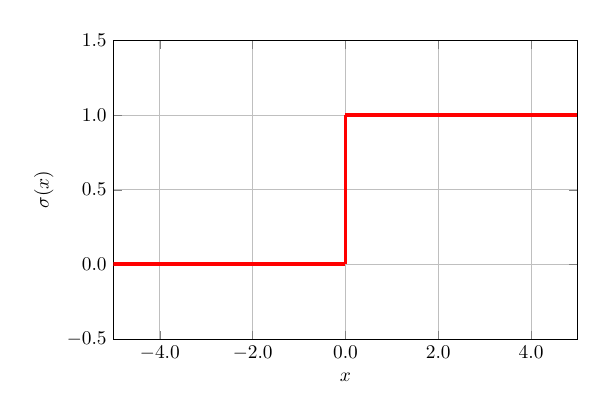
\begin{tikzpicture}[scale=0.70]
    \begin{axis}[
        width=10cm, height=7cm,
        xmin=-5, xmax=5,
        ymin=-0.5, ymax=1.5, 
        grid, 
        xlabel=$x$, ylabel=$\sigma(x)$,
        xtick = {-4.0,-2.0,0,2.0,4.0},
        ytick = {-0.5,0,0.5,1.0,1.5},
        y tick label style={/pgf/number format/.cd,%
                fixed,
                fixed zerofill,
                precision=1},
        x tick label style={/pgf/number format/.cd,%
                fixed,
                fixed zerofill,
                precision=1}
        ]
        
        \draw[line width=2.pt,color=red] (-5,0) -- (0,0);
        \draw[line width=2.pt,color=red] (0,0) -- (0,1);
        \draw[line width=2.pt,color=red] (0,1) -- (5,1);
        
    \end{axis}
\end{tikzpicture}
        \caption{Heaviside}
        \label{fig:activation:a}
    \end{subfigure}%
    \hfill
    \begin{subfigure}[b]{0.5\textwidth}
        \centering 
        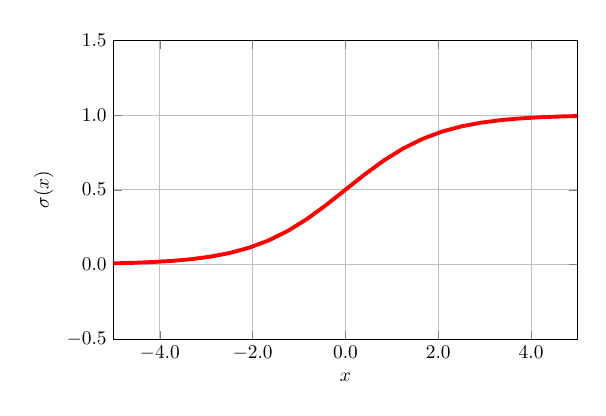
\begin{tikzpicture}[scale=0.70]
    \begin{axis}[
        width=10cm, height=7cm,
        xmin=-5, xmax=5,
        ymin=-0.5, ymax=1.5, 
        grid, 
        xlabel=$x$, ylabel=$\sigma(x)$,
        xtick = {-4.0,-2.0,0,2.0,4.0},
        ytick = {-0.5,0,0.5,1.0,1.5},
        y tick label style={/pgf/number format/.cd,%
                fixed,
                fixed zerofill,
                precision=1},
        x tick label style={/pgf/number format/.cd,%
                fixed,
                fixed zerofill,
                precision=1}
        ]
        
        \addplot[line width=2.pt,color=red]{1/(1+e^(-x))};
    
    \end{axis}
\end{tikzpicture}
        \caption{Sigmoid}
        \label{fig:activation:b}
    \end{subfigure}%
    \\
    \begin{subfigure}[b]{0.5\textwidth}
        \centering 
		  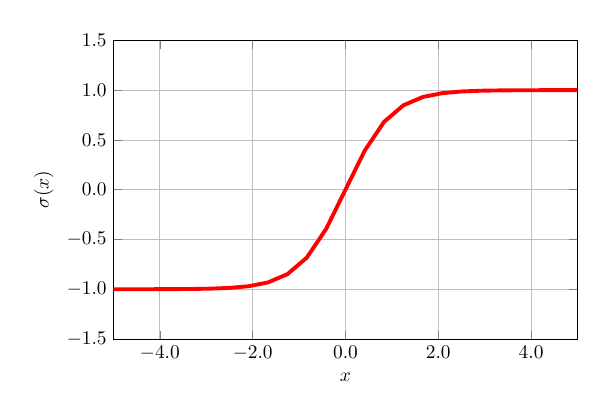
\begin{tikzpicture}[scale=0.70]
    \begin{axis}[
        width=10cm, height=7cm,
        xmin=-5, xmax=5,
        ymin=-1.5, ymax=1.5, 
        grid, 
        xlabel=$x$, ylabel=$\sigma(x)$,
        xtick = {-4.0,-2.0,0,2.0,4.0},
        ytick = {-1.5,-1.0,...,1.5},
        y tick label style={/pgf/number format/.cd,%
                fixed,
                fixed zerofill,
                precision=1},
        x tick label style={/pgf/number format/.cd,%
                fixed,
                fixed zerofill,
                precision=1}
        ]
        
        \addplot[line width=2.pt,color=red]{tanh(x)};
    
    \end{axis}
\end{tikzpicture}
        \caption{Hyperbolic tangent}
        \label{fig:activation:c}
    \end{subfigure}%
    \hfill
    \begin{subfigure}[b]{0.5\textwidth}
        \centering 
        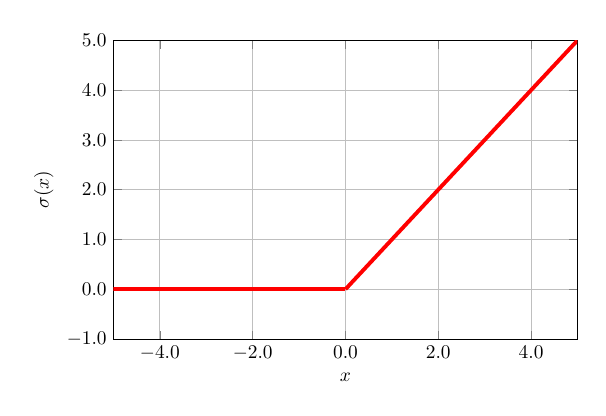
\begin{tikzpicture}[scale=0.70]
    \begin{axis}[
        width=10cm, height=7cm,
        xmin=-5, xmax=5,
        ymin=-1.0, ymax=5.0, 
        grid, 
        xlabel=$x$, ylabel=$\sigma(x)$,
        xtick = {-4.0,-2.0,0,2.0,4.0},
        ytick = {-1.0,0.0,...,5.0},
        y tick label style={/pgf/number format/.cd,%
                fixed,
                fixed zerofill,
                precision=1},
        x tick label style={/pgf/number format/.cd,%
                fixed,
                fixed zerofill,
                precision=1}
        ]
        
        \draw[line width=2.pt,color=red] (-5,0) -- (0,0);
        \addplot[line width=2.pt,color=red,domain=0:5]{x};
    
    
    \end{axis}
\end{tikzpicture}
        \caption{Rectified linear unit}
        \label{fig:activation:d}
    \end{subfigure}%
    \caption{Examples of the most used activation functions}
    \label{fig:activation}
\end{figure}

The sigmoid, or logistic activation function, (\autoref{fig:activation:b}) is probably the most famous of all. The main
reason why it is so widely used is that it returns values between $0$ and $1$. Therefore, since the probability
exists only in that specific range, it is especially used for models predicting a certain probability, given by network
output. Similarly, another possible choice is the hyperbolic tangent (\autoref{fig:activation:c}): the advantage over
the sigmoid is that negative inputs are mapped strongly negative and zero inputs are mapped near zero. The ReLU
activation (\autoref{fig:activation:d}), on the other hand, appears to have a completely different shape compared to the
previous. Moreover, it is not limited, ranging from $0$ to infinity. The downside of this particular activation is the
inappropriate mapping of negative values, since it turns every negative input value into zero. 

It has to be stressed that selecting the right activation function is crucial in order to achieve excellent results and speed
up the computation. For this reason, it is useful to use different activation functions among the layers, depending on
the particular layer purpose.

\subsection{Loss function}

In the context of algorithmic optimization, the function implemented to evaluate a candidate solution (i.e. a set of
parameters) is called objective function. Such function is either maximized or minimized, meaning that the optimization
search converges to the candidate solution that evaluates to the higher or lower value of the objective function
respectively. In the context of neural networks, the objective function is often referred to as "loss" function or
"cost" function, as it is more common to seek to minimize the error of the network. As a matter of fact, the loss
function serves the purpose of quantifying how much the network predictions are wrong: the set free parameters
$(\hat{\mathbf{w}},\,\vec{b})$ that evaluates to the minimum of the loss function are chosen to be the best parameters
of the network. Some of the most used cost functions are the Mean Absolute Error, Mean Square Error, Cross Entropy Loss
and KL Divergence. However, when dealing with a very specific problem it is suggested to build a loss function ad hoc
for that particular work. 